
\section{Mapping}

The quality of the maps are investigated after a complete exploration of the environment without object search. This was done in all three environments multiple times. In this section typical results of those exploration runs are presented and also encountered problems. At first the metric maps are investigated, followed by the Room-Type-Maps and the Object-Maps. At the end of this section the resulting Object-Probability-Maps and the total object probabilities are discussed.

\subsection{Hybrid Metric Map} \label{EvalMapping}

In figure \ref{map2d_home}, figure \ref{map2d_lab} and figure \ref{map2d_ist} maps created in the three environments are shown. The 2D maps of the rooms have in general good quality, especially in the small rooms. All maps contain cells wrongly set to free outside of the room. On the one hand those are caused by reflexion and transparent surfaces. On the other hand they are caused by the handling of invalid range measurements described in section \ref{preprocessing}. However those cause no major problems. The maps of the rooms lab1 and institute1 are distorted. In the map of room lab1 the top part leans to the left while the bottom right part is rotated towards the bottom right part. In the map of room institute1 the bottom corridor is curved upwards. The distortion in both rooms are probably caused by a conjunction of inaccurate odometry and insufficient distinct features in the visible by the LIDAR. These distortion show the benefit of the hybrid map design. The maps are still sufficiently accurate, but those distortion become more and more problematic with larger maps. As can be seen in the maps the doorway poses are all quiet accurate. 

\begin{figure}
\centering
  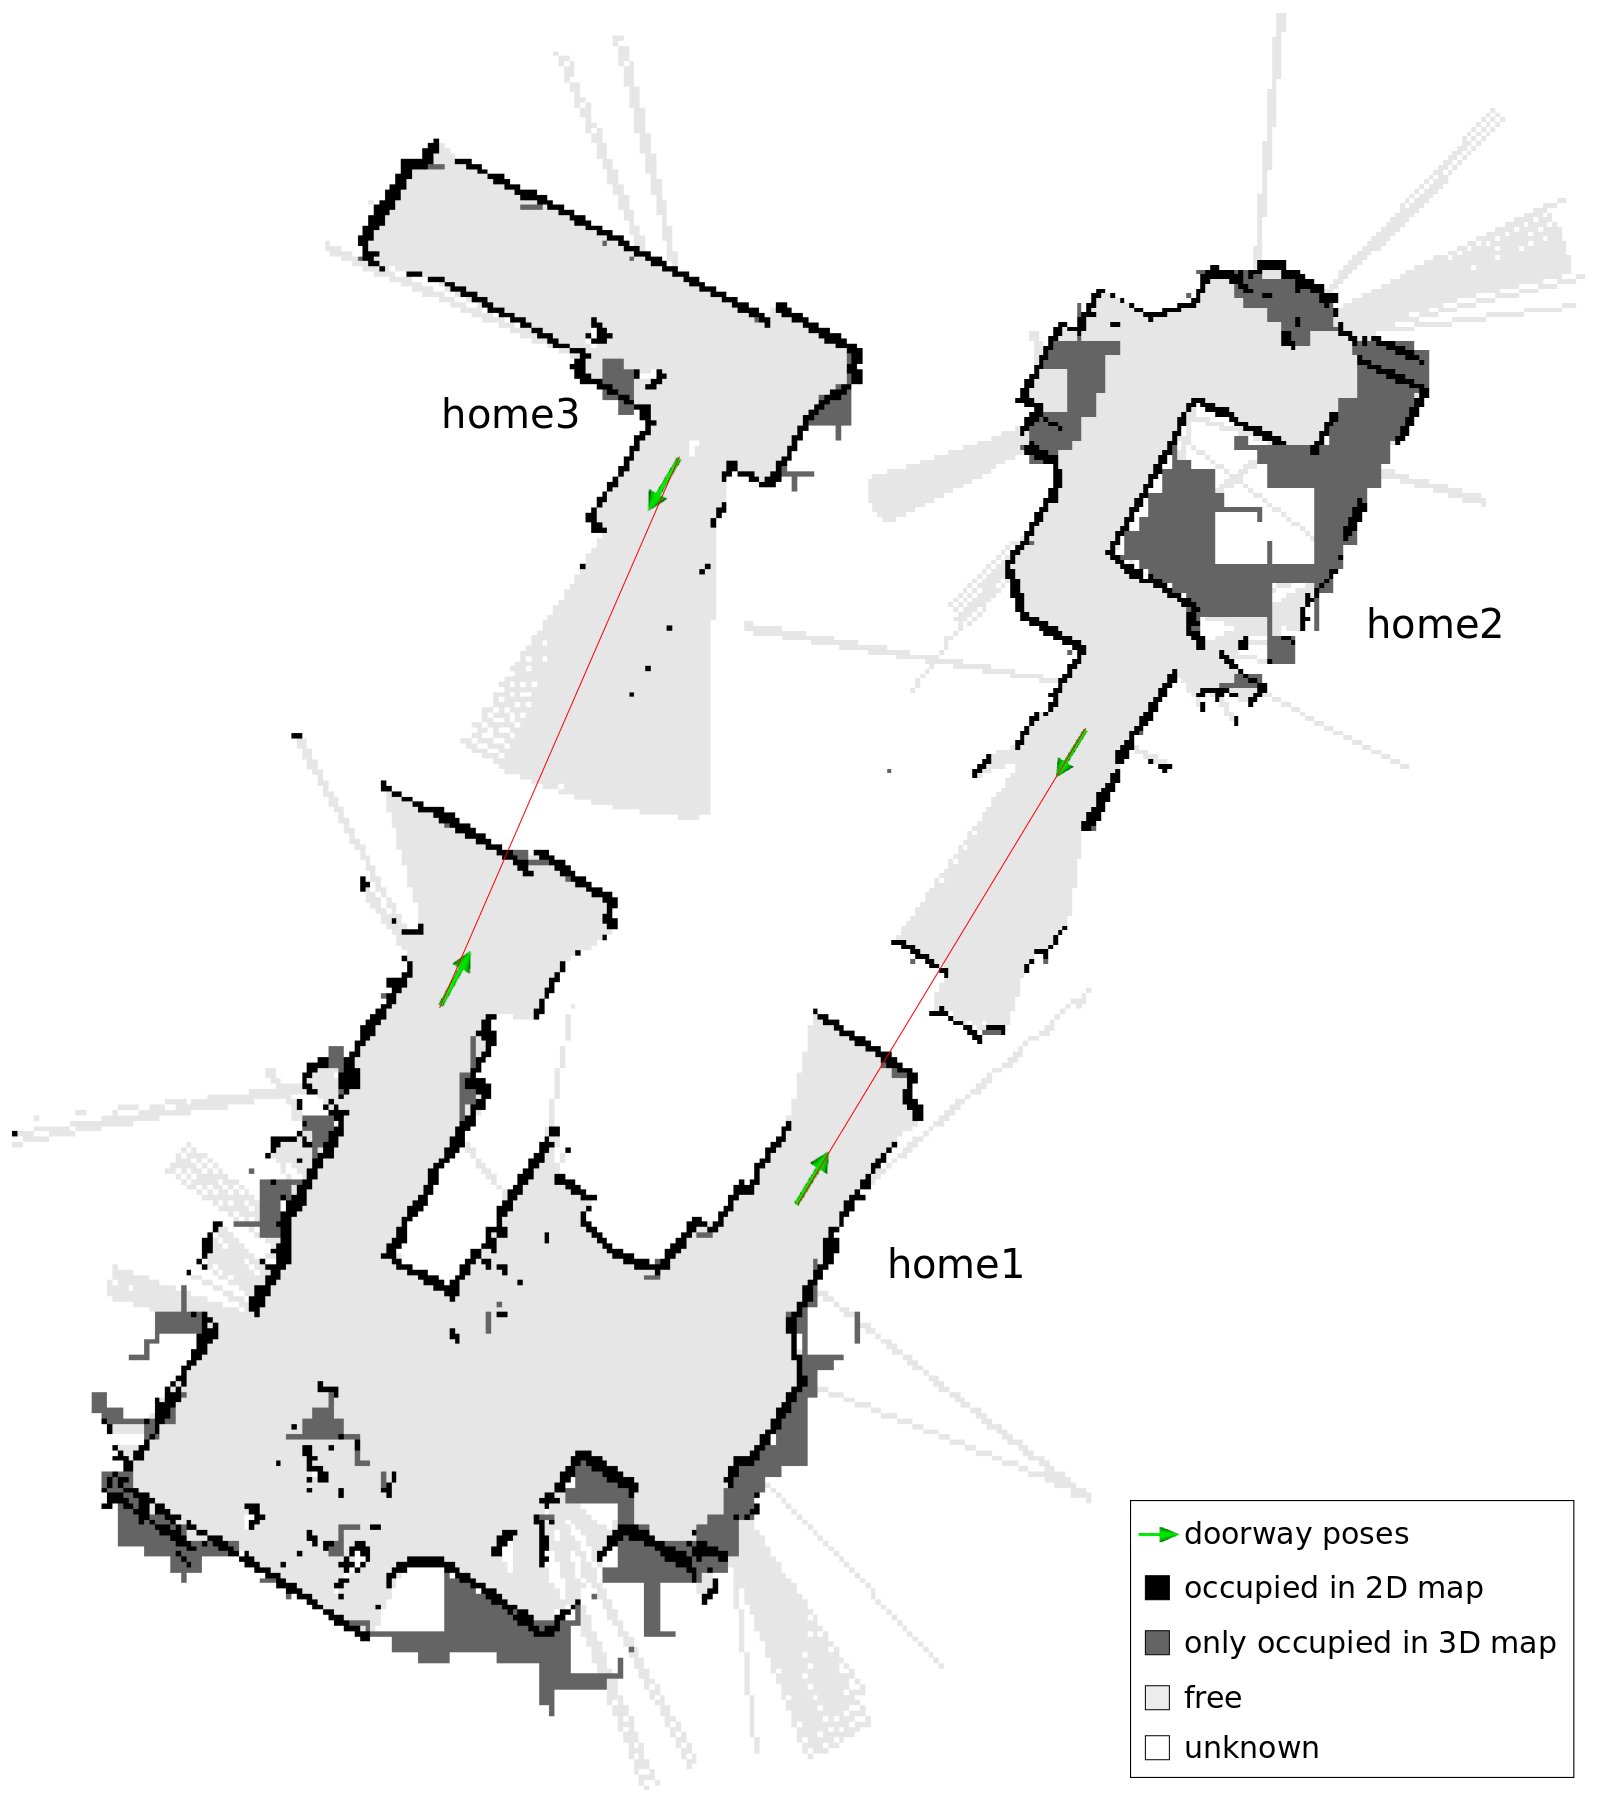
\includegraphics[width=0.9\textwidth,clip]{figures/2Dmaps/all5.png}
  \caption[Hybrid map of the home environment]{Hybrid map of the home environment: The room home1 is combination of a kitchen and a living room, the room home2 is a bedroom with an office-like area in the upper right corner and the room home3 is an anteroom.}
  \label{map2d_home}
\end{figure}

\begin{figure}
\centering
  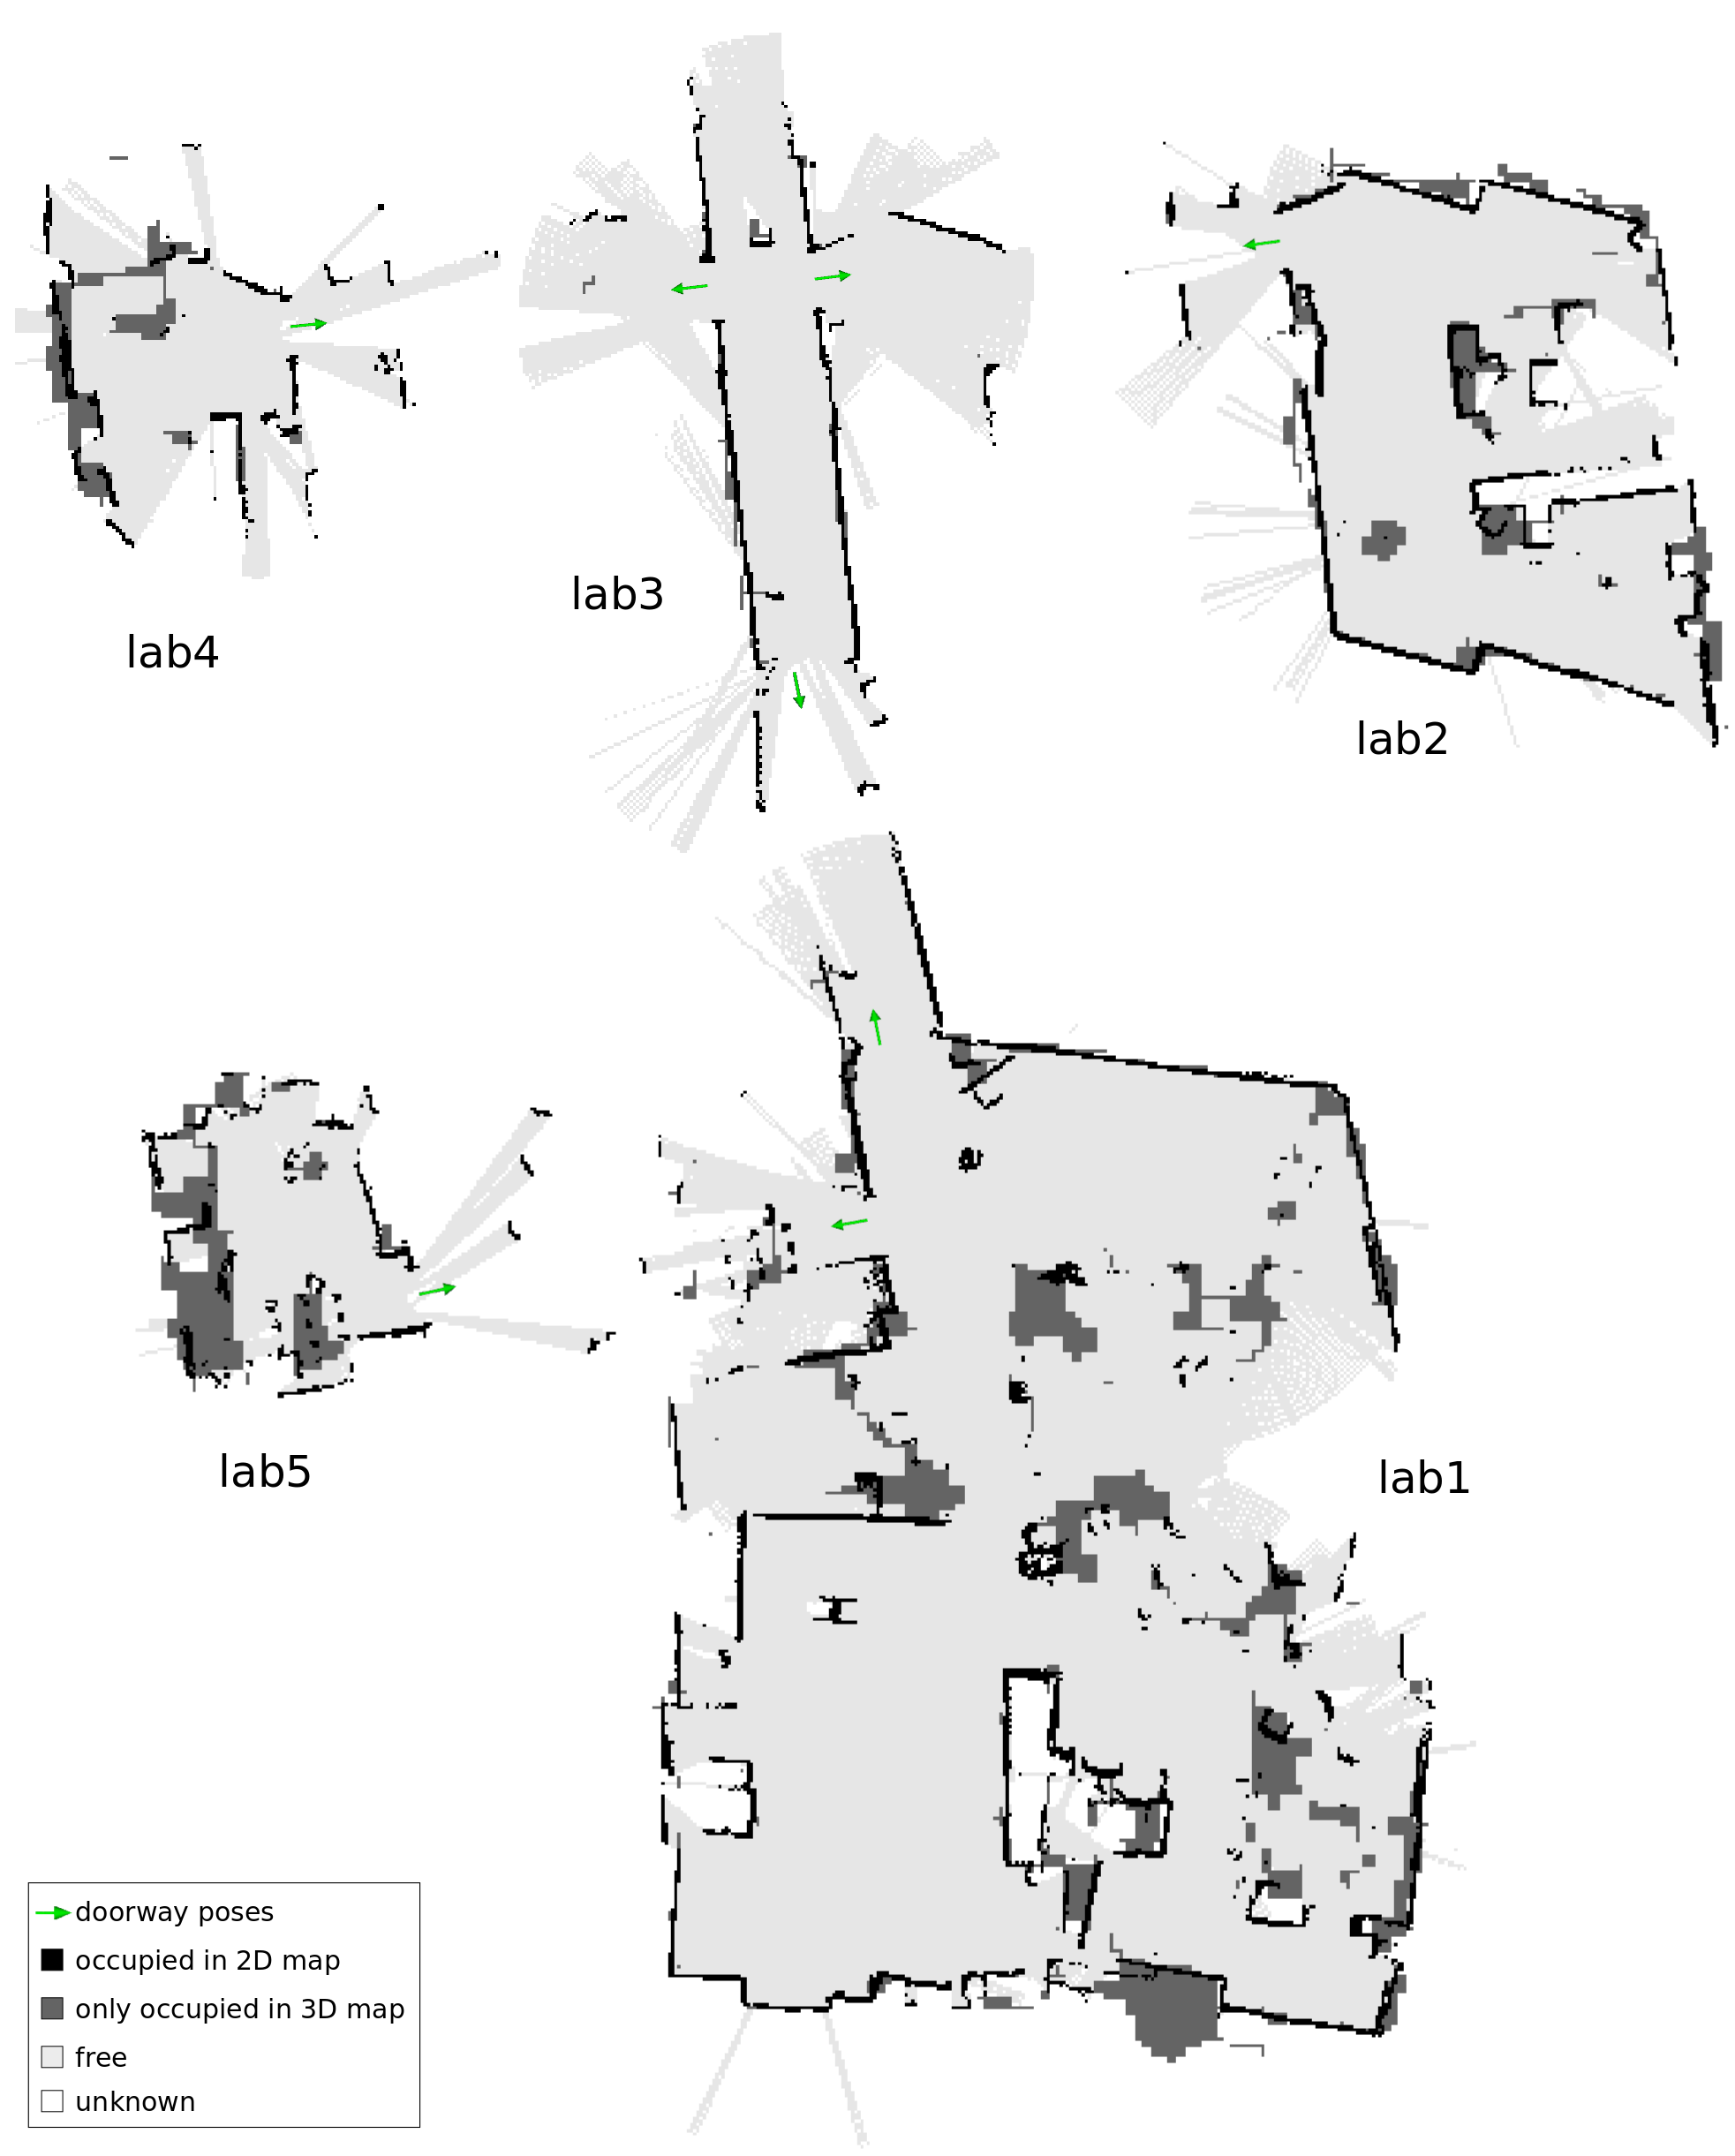
\includegraphics[width=0.99\textwidth,clip]{figures/2Dmaps/all_lab.png}
  \caption[Hybrid map of the robotics-lab environment]{Hybrid map of robotics-lab environment: The room lab1 is the robotics-lab, which consists mainly of an office area and has free space at the botton left and a sofa and a kitchen area at the bottom right. The room lab2 is an office, the room lab3 is a corridor, the room lab4 is also an office and the room lab5 is a workshop/storage room.}
  \label{map2d_lab}
\end{figure}

\begin{figure}
\centering
  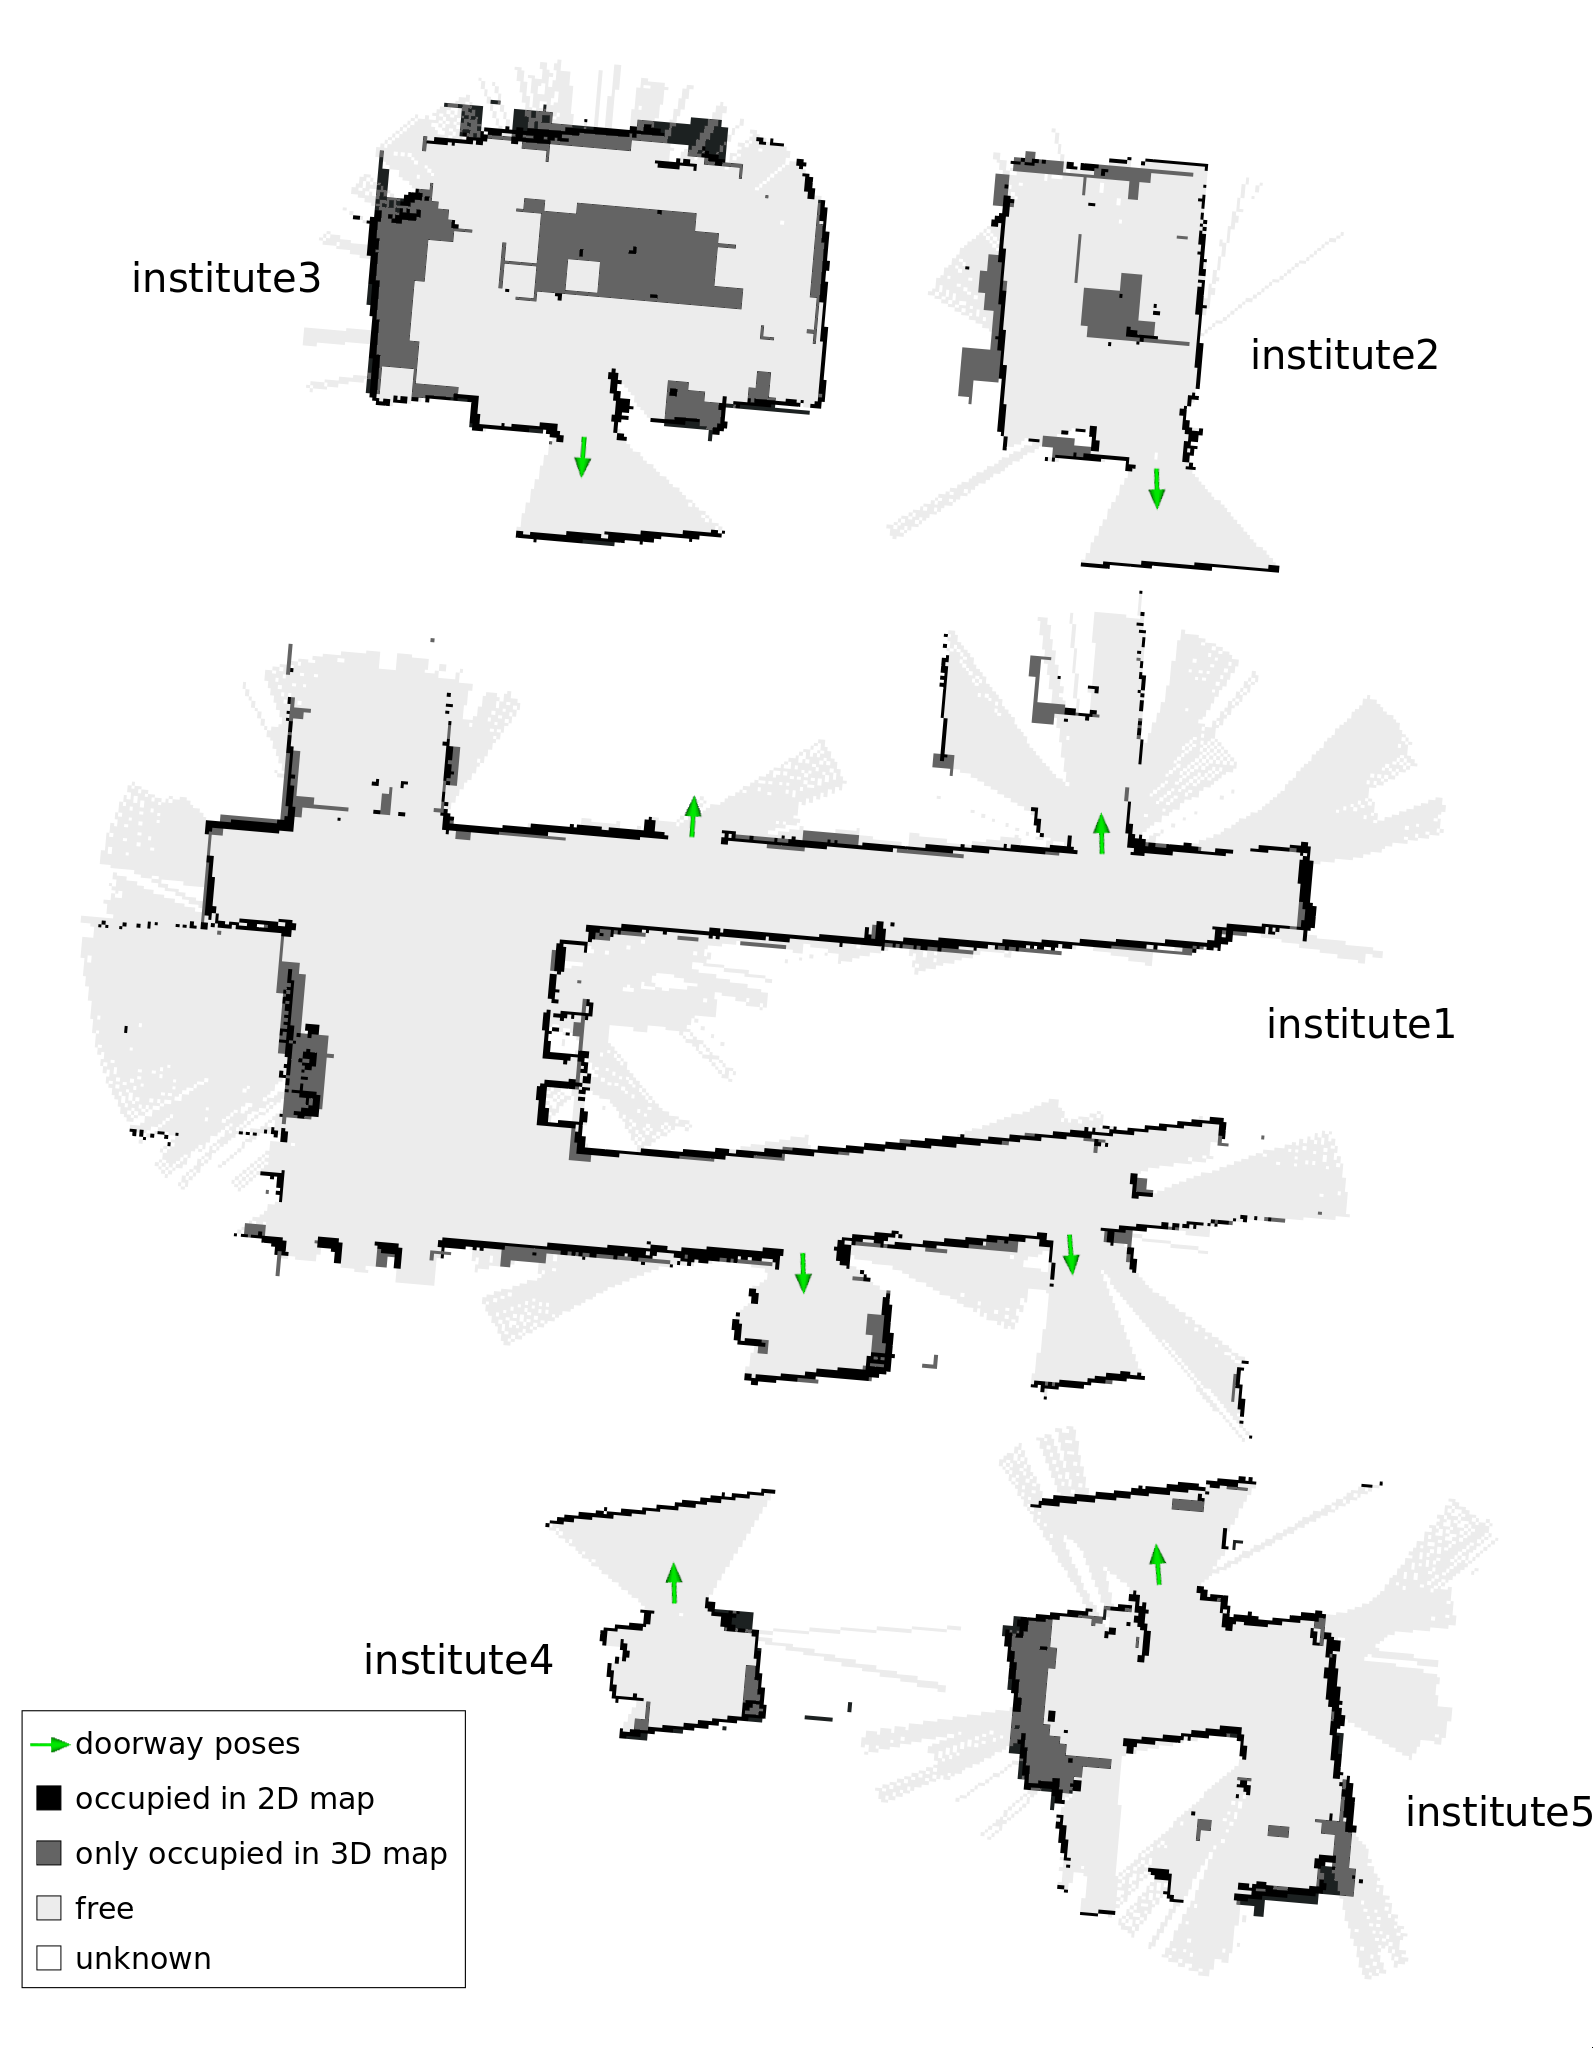
\includegraphics[width=0.9\textwidth,clip]{figures/2Dmaps/all_IST_b.png}
  \caption[Hybrid map of the university floor]{Hybrid map of a part of an university floor: The room institute1 is a corridor with an copy area, the room institute2 contains a kitchen area and a dining table, the room institute3 is a meeting room, the room institute4 is a bathroom and the room institute5 is a secretariat. }
  \label{map2d_ist}
\end{figure}

\subsection{Room Type Map}

\begin{figure}
\renewcommand*\thesubfigure{\arabic{subfigure}} 
\centering
\begin{tabular}{cc}
\subfloat[]{
\includegraphics[width=0.45\textwidth]{figures/wz_imgs/1.png}} &
\subfloat[]{
\includegraphics[width=0.45\textwidth]{figures/wz_imgs/2.png}} \\
\subfloat[]{
\includegraphics[width=0.45\textwidth]{figures/wz_imgs/3.png}} &
\subfloat[]{
\includegraphics[width=0.45\textwidth]{figures/wz_imgs/4.png}} \\
\subfloat[]{
\includegraphics[width=0.45\textwidth]{figures/wz_imgs/5.png}} &
\subfloat[]{
\includegraphics[width=0.45\textwidth]{figures/wz_imgs/6.png}}
\end{tabular}
\caption[Images of the room home1]{Images with place classification results of the room home1}
\label{wz_imgs}
\end{figure}

\begin{figure}
\centering
  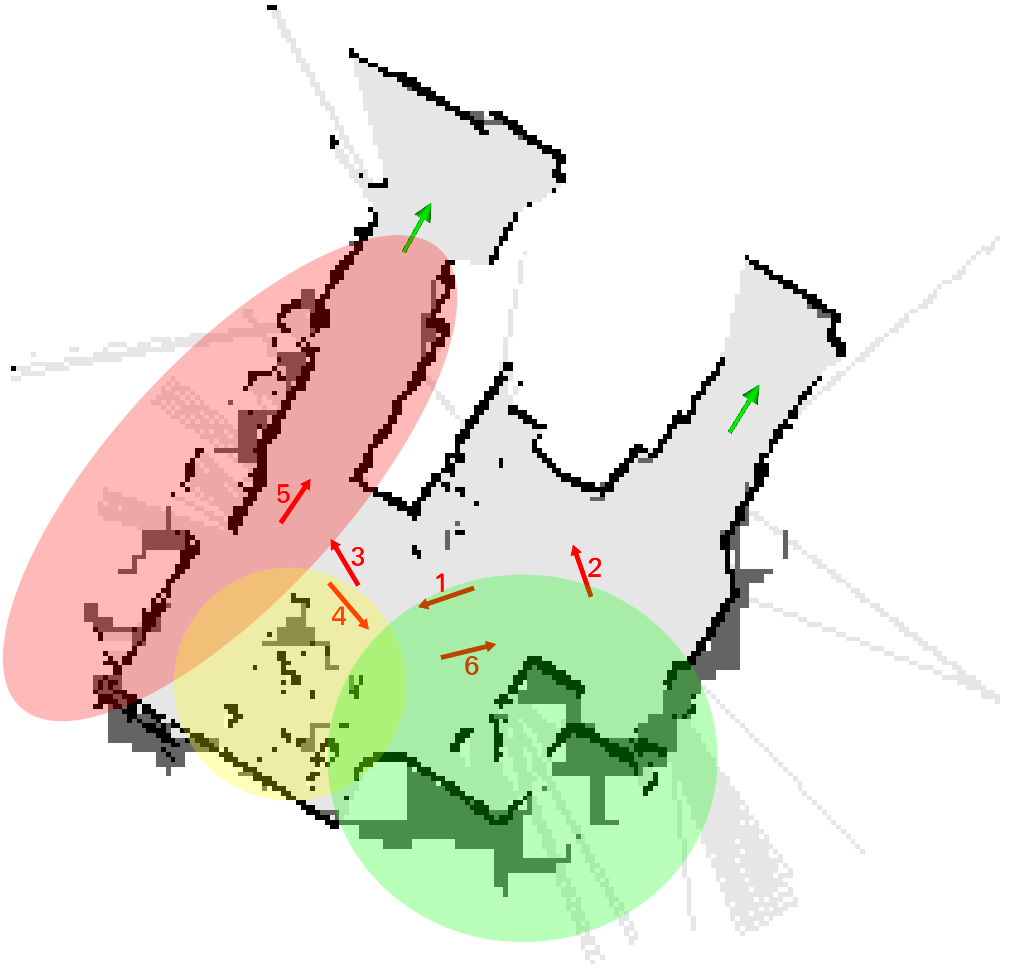
\includegraphics[width=0.9\textwidth, trim=0 0 50 0,clip]{figures/wz_imgs/wz_views_b.png}
  \caption[Detailed map of the room home1 with image poses]{Detailed map of the room home1: Green arrows mark the doorways, the numbered red arrows are the view poses of the corresponding images from figure \ref{wz_imgs}}.
  \label{wz_views}
\end{figure}

\begin{figure}
\centering
\begin{tabular}{ccc}
\subfloat[run 1]{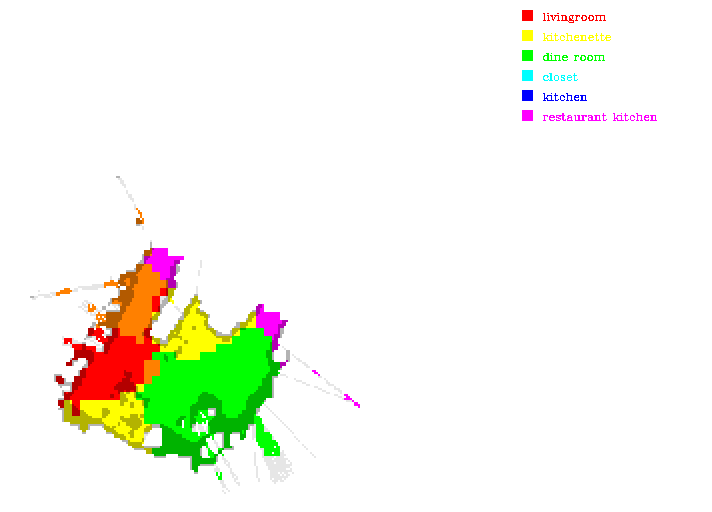
\includegraphics[width=0.3\textwidth,trim=40 10 360 250, clip]{figures/wz_imgs/h5e/classes_0_b.png}} &
\subfloat[run 1, without room type correlation]{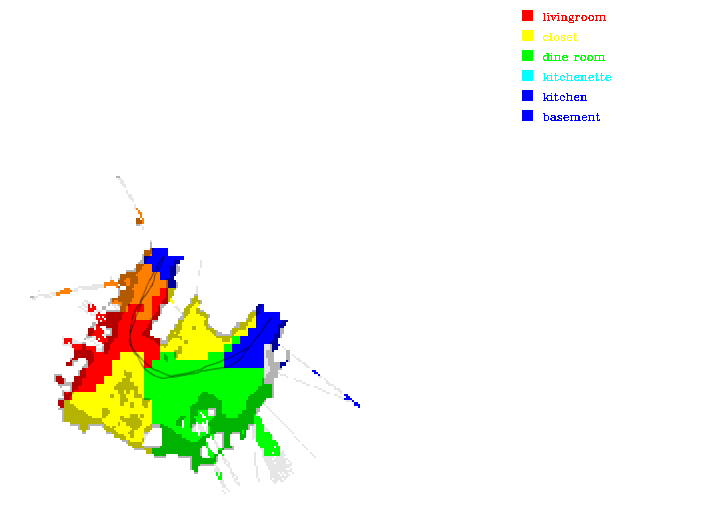
\includegraphics[width=0.3\textwidth,trim=40 10 360 250, clip]{figures/wz_imgs/h5e/classes_1_b.png}} &
\subfloat[run 2]{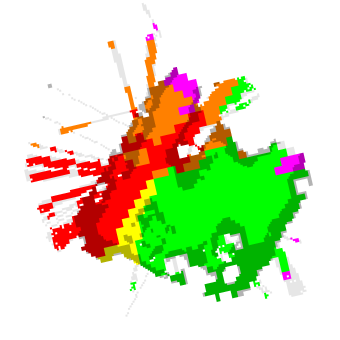
\includegraphics[width=0.3\textwidth,trim=0 20 0 50,clip]{figures/wz_imgs/h5e/classes_2_b_b2.png}} \\
\subfloat[run 3]{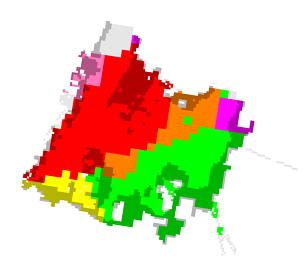
\includegraphics[width=0.3\textwidth,trim=30 0 0 50,clip]{figures/wz_imgs/h5e/classes_3_b.png}} &
\subfloat[after executed search]{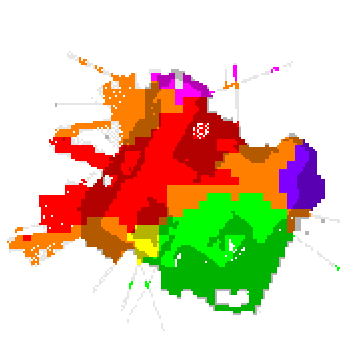
\includegraphics[width=0.3\textwidth,trim=0 0 0 50,clip]{figures/wz_imgs/h5e/classes_search_b.png}} &
\subfloat{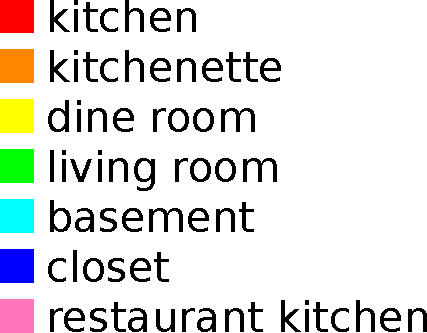
\includegraphics[width=0.3\textwidth,trim=-50 0 0 0, clip]{figures/wz_imgs/h5e/legend.pdf}} 
\end{tabular}
\caption[Map of most likely room types for the room home1]{Map of most likely room types for the room home1}
\label{frontier_calc}
\end{figure}

\begin{figure}
\centering
\begin{tabular}{ccc}
\subfloat[kitchen]{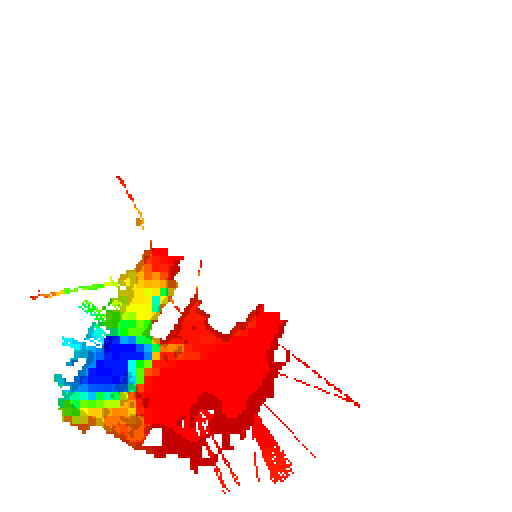
\includegraphics[width=0.3\textwidth,trim=40 10 160 250, clip]{figures/wz_imgs/h5e/kitchen_b.png}} & 
\subfloat[kitchenette]{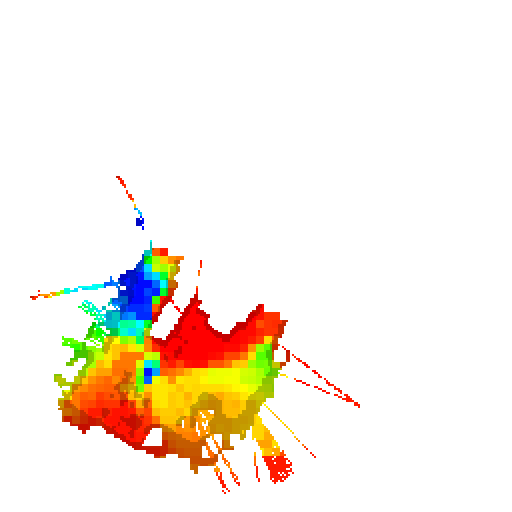
\includegraphics[width=0.3\textwidth,trim=40 10 160 250, clip]{figures/wz_imgs/h5e/kitchenette_b.png}} &
\subfloat[living room]{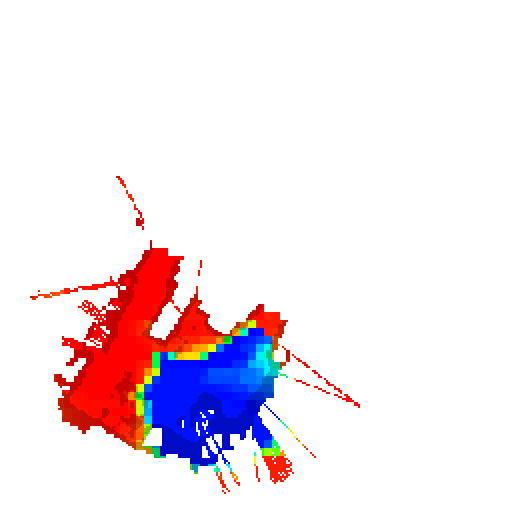
\includegraphics[width=0.3\textwidth,trim=40 10 160 250, clip]{figures/wz_imgs/h5e/livingroom_b.png}} \\
\subfloat[dine room]{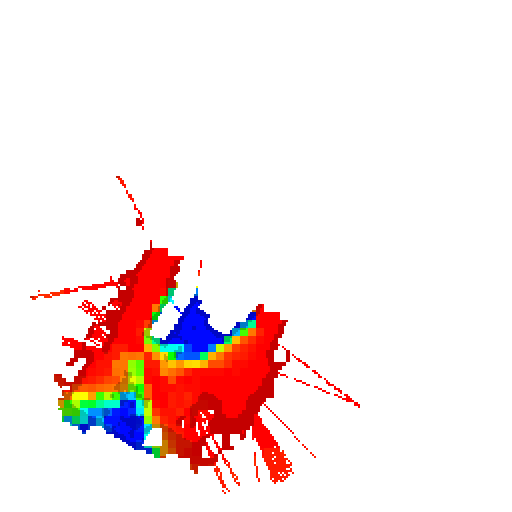
\includegraphics[width=0.3\textwidth,trim=40 10 160 250, clip]{figures/wz_imgs/h5e/dine_b.png}} &
\subfloat[closet]{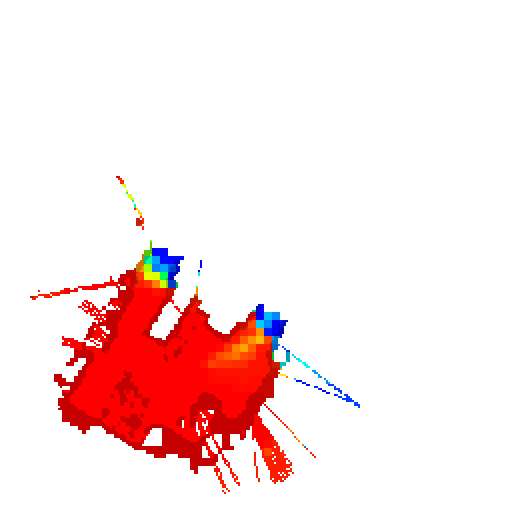
\includegraphics[width=0.3\textwidth,trim=40 10 160 250, clip]{figures/wz_imgs/h5e/closet_b.png}} &
\subfloat{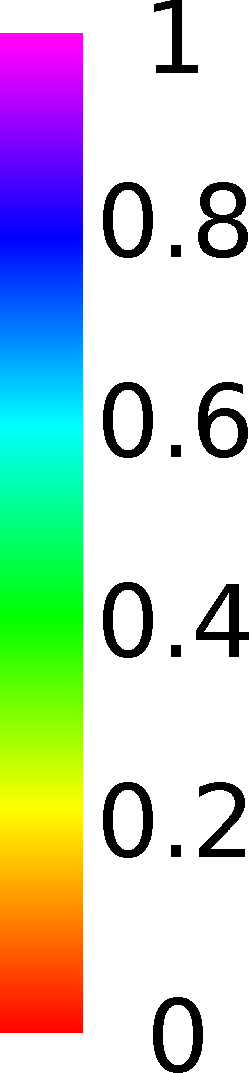
\includegraphics[width=0.3\textwidth,trim=-300 0 -300 0, clip]{figures/wz_imgs/h5e/problegend.pdf}} 
\end{tabular}
\caption{Probabilities of stated room type in room home 1}
\label{frontier_calc}
\end{figure}

\subsection{Object Map}



\subsection{Information after Peek Task}

\begin{figure}
\centering
\begin{tabular}{ccc}
\subfloat[office: 0.4442 \newline home office: 0.3214 \newline attic: 0.0174]{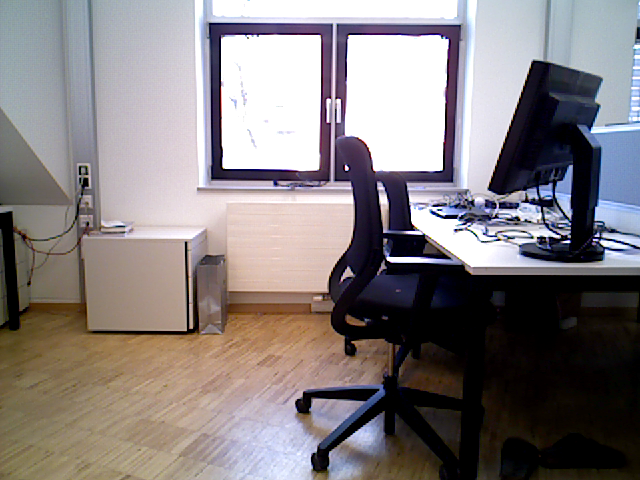
\includegraphics[width=0.4\textwidth, clip]{figures/peek/explore_lab_1bag1221.png}} &
\subfloat[dining room: 0.3918 \newline livingroom: 0.3093 \newline closet: 0.0878]{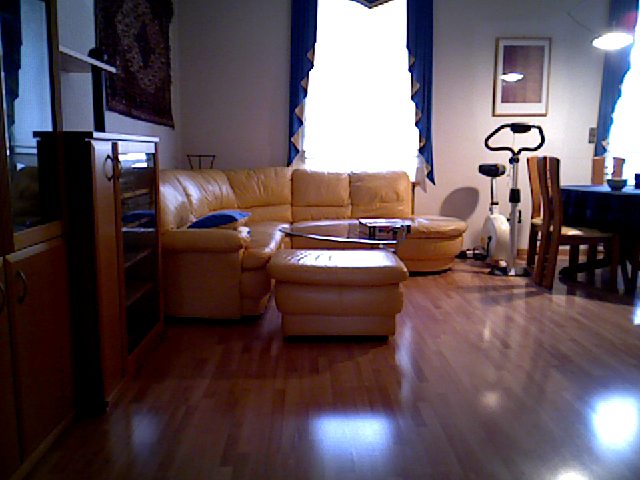
\includegraphics[width=0.4\textwidth, clip]{figures/peek/h5ebag117.png}} \\
\subfloat[kitchen: 0.4841 \newline restaurant kitchen: 0.2690 \newline kitchenette: 0.0439]{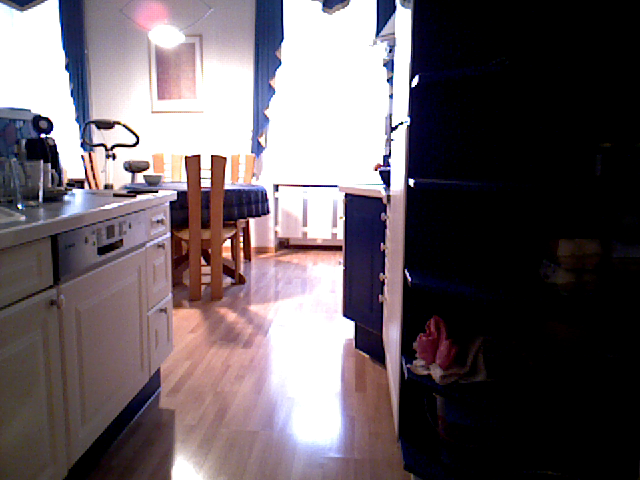
\includegraphics[width=0.4\textwidth, clip]{figures/peek/h7ebag41.png}} &
\subfloat[kitchen: 0.3211 \newline dining room: 0.2779 \newline restaurant kitchen: 0.0978]{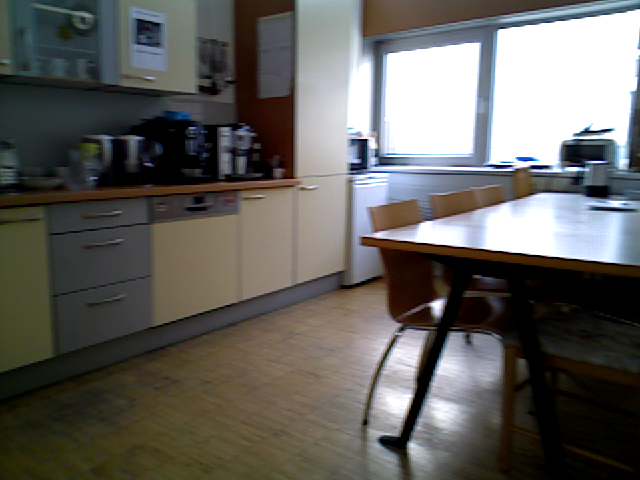
\includegraphics[width=0.4\textwidth, clip]{figures/peek/IST_explore_subag470.png}} \\
\subfloat[shower: 0.7556 \newline locker room: 0.1701 \newline martial arts gym: 0.0038]{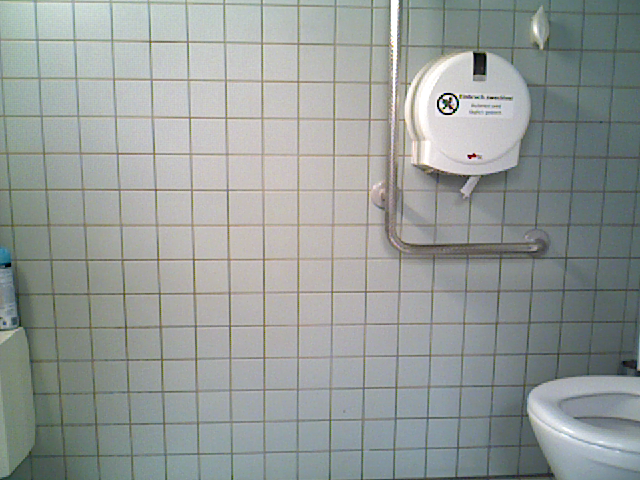
\includegraphics[width=0.4\textwidth, clip]{figures/peek/IST_explore_subag148.png}} &
\subfloat[classroom: 0.6971 \newline cafeteria: 0.0919 \newline conference center: 0.0256]{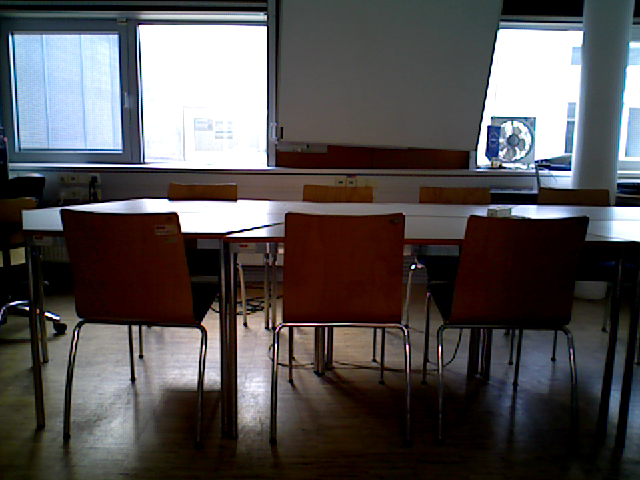
\includegraphics[width=0.4\textwidth, clip]{figures/peek/IST_explore_subag850.png}} 
\end{tabular}
\caption{Calculation of the frontiers: In those binary images black is 1 and white is 0; the gray accessible area in the last image is just for clarity}
\label{frontier_calc}
\end{figure}